\documentclass[conference]{IEEEtran}
\IEEEoverridecommandlockouts

\usepackage[utf8]{inputenc}
\usepackage[english]{babel}
\usepackage[T1]{fontenc}
\usepackage{cite}
\usepackage{amsmath,amssymb,amsfonts}
\usepackage{algorithmic}
\usepackage{graphicx}
\usepackage{textcomp}
\usepackage{xcolor}
\usepackage{booktabs}
\usepackage{placeins}
\def\BibTeX{{\rm B\kern-.05em{\sc i\kern-.025em b}\kern-.08em
    T\kern-.1667em\lower.7ex\hbox{E}\kern-.125emX}}

\usepackage[labelsep=endash]{caption}
\renewcommand{\figurename}{Fig.}

% Figures are generated by the notebook into yoga-pose-classification/doc/img/ — copy them here
\graphicspath{{img/}}


\begin{document}

\title{Yoga Pose Classification Using Transfer Learning on the Yoga-82 Dataset}

\author{
\IEEEauthorblockN{Martin Martijan}
\IEEEauthorblockA{\textit{Faculty of Mathematics and Informatics}\\
Vilnius, Lithuania \\
martin.martijan@mif.vu.lt}
\and
\IEEEauthorblockN{Arnas Vaicekauskas}
\IEEEauthorblockA{\textit{Faculty of Mathematics and Informatics}\\
Vilnius, Lithuania \\
arnas.vaicekauskas@mif.stud.vu.lt}

}

\maketitle

\begin{abstract}
We address the problem of fine-grained yoga pose classification across 82 categories using the Yoga-82 benchmark dataset. A pretrained EfficientNet-B0 model is fine-tuned end-to-end with class-weighted cross-entropy loss, cosine annealing learning rate scheduling, and standard data augmentation. The resulting model achieves 85.09\% top-1 accuracy on the test set and a macro-averaged F1 score of 0.84 across all 82 classes. Beyond classification, we demonstrate that the 1280-dimensional average-pooled embeddings support effective cosine similarity image retrieval, returning visually coherent pose matches for arbitrary query images. Error analysis identifies visually ambiguous and underrepresented poses as the primary source of failure.
\end{abstract}

\begin{IEEEkeywords}
yoga pose classification, transfer learning, EfficientNet, fine-grained recognition, image retrieval
\end{IEEEkeywords}


\section{Introduction}

Automatic recognition of human poses from photographs is a challenging computer vision problem. When restricted to yoga postures, the task becomes a fine-grained classification problem: the model must resolve subtle differences in body orientation, limb position, and depth perspective while remaining robust to wide variation in image conditions (lighting, background, clothing, body type). Accurate pose classification has practical value in fitness coaching applications, rehabilitation monitoring, and interactive training platforms.

The Yoga-82 dataset~\cite{verma2020yoga} was introduced specifically to benchmark this problem at a fine-grained scale, providing 82 yoga pose categories with real-world photographic images. The combination of high intra-class variation and inter-class visual similarity (many poses share partial body configurations) makes Yoga-82 a significantly harder benchmark than broad action recognition datasets.

Deep convolutional networks trained with transfer learning have become the dominant approach for image classification tasks where labeled data is limited relative to model capacity~\cite{lecun2015deep}. In this work we adopt EfficientNet-B0~\cite{tan2019efficientnet} pretrained on ImageNet as our backbone. We fine-tune the full network end-to-end, applying class-weighted loss to mitigate label imbalance and cosine annealing scheduling to smooth convergence. We additionally demonstrate that the learned embeddings support visual similarity search, providing an interpretable window into the model's internal representation of pose space.


\section{Data}

\subsection{Dataset}

The Yoga-82 dataset~\cite{verma2020yoga} organizes 82 yoga pose categories into a three-level semantic hierarchy, but in this work we treat the problem as flat 82-class classification. We use the official dataset split. Table~\ref{tab:dataset} summarizes the image counts and average resolutions per split.

\begin{table}[htbp]
\caption{Yoga-82 dataset split summary}
\begin{center}
\begin{tabular}{|l|c|c|c|}
\hline
\textbf{Split} & \textbf{Images} & \textbf{Classes} & \textbf{Avg.\ resolution (px)} \\
\hline
Train      & 11{,}652 & 82 & $744 \times 622$ \\
Validation &  3{,}351 & 82 & $761 \times 633$ \\
Test       &  1{,}764 & 82 & $777 \times 618$ \\
\hline
\end{tabular}
\label{tab:dataset}
\end{center}
\end{table}

Image dimensions vary considerably: training set widths range from 1 to 6{,}240 pixels. The dataset is also class-imbalanced, with sample counts per class ranging from a handful to several dozen in the training split.

% FIGURE NEEDED: fig_class_dist.png
% Plot: bar chart of samples-per-class in the training split, sorted descending.
% Purpose: visually demonstrates the class imbalance that motivates class-weighted loss.
\begin{figure}[htbp]
\centerline{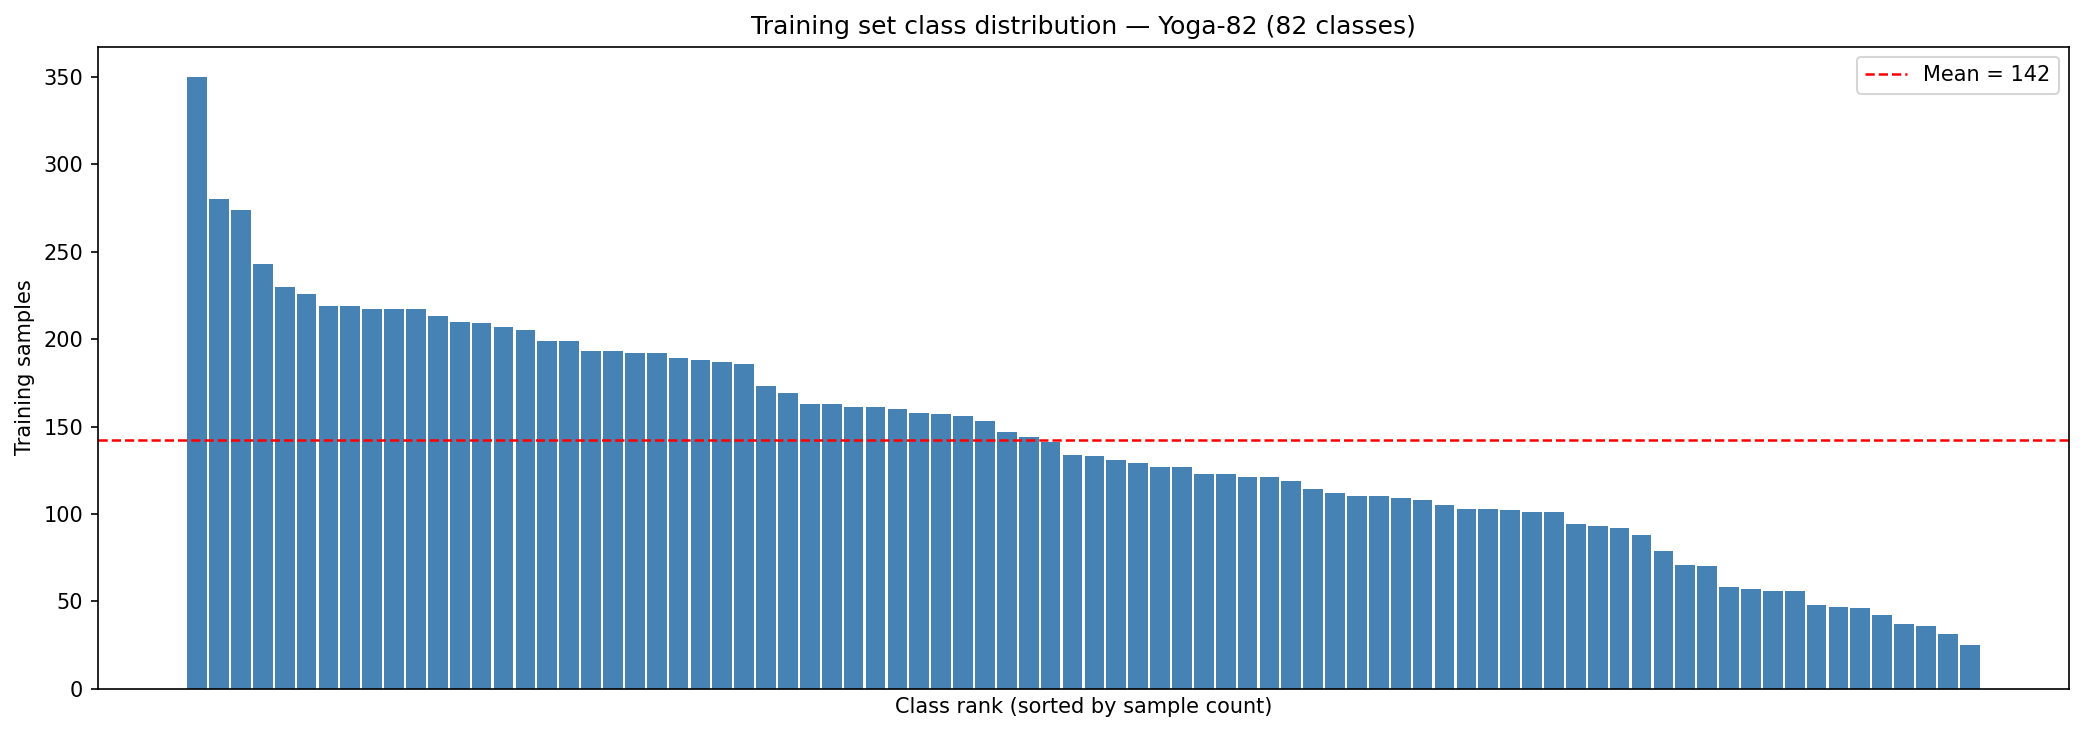
\includegraphics[width=\columnwidth]{fig_class_dist.png}}
\caption{Training set sample count per class, sorted in descending order. Class imbalance motivates the use of weighted cross-entropy loss.}
\label{fig:class_dist}
\end{figure}

\subsection{Preprocessing}

All images are resized so that the shorter dimension becomes 440 pixels. Training images then undergo a random $384\times384$ crop; validation and test images use a deterministic center crop of the same size. Pixel values are normalized with ImageNet channel statistics ($\mu = [0.485, 0.456, 0.406]$, $\sigma = [0.229, 0.224, 0.225]$).

Training-time augmentation includes: random horizontal flip, random rotation up to $\pm15^\circ$, and color jitter (brightness $\pm0.3$, contrast $\pm0.3$, saturation $\pm0.2$). No augmentation other than deterministic center crop and normalization is applied at inference.

% FIGURE NEEDED: fig_samples.png
% Plot: 4x4 or 5x5 grid showing one representative image per selected class,
%        with class name as subtitle under each image.
% Purpose: gives the reader a concrete sense of the pose variety and intra-class
%          visual diversity in the dataset.


\section{Methods}

\subsection{Model Architecture}

We use EfficientNet-B0~\cite{tan2019efficientnet} as the backbone, initialized from publicly available ImageNet~\cite{deng2009imagenet} pretrained weights. EfficientNet-B0 applies compound scaling — simultaneously increasing network depth, width, and input resolution — to achieve a favorable accuracy-efficiency balance. The original 1000-class classification head is replaced with a single linear layer:

\begin{equation}
\hat{y} = W\,\mathbf{z} + b, \quad W \in \mathbb{R}^{82 \times 1280},
\label{eq:classifier}
\end{equation}

where $\mathbf{z} \in \mathbb{R}^{1280}$ is the average-pooled feature vector extracted by the backbone. All layers including the backbone are trained end-to-end.

\subsection{Loss Function}

The dataset is class-imbalanced, so we use weighted cross-entropy. The weight assigned to class $c$ is:

\begin{equation}
w_c = \frac{N}{C \cdot n_c},
\label{eq:classweight}
\end{equation}

where $N$ is the total number of training samples, $C = 82$ is the number of classes, and $n_c$ is the number of training samples for class $c$. The training objective is then:

\begin{equation}
\mathcal{L} = -\frac{1}{N} \sum_{i=1}^{N} w_{y_i} \log p\!\left(y_i \mid x_i\right).
\label{eq:loss}
\end{equation}

Rare classes receive larger weights, encouraging the model to attend to underrepresented poses.

\subsection{Optimization}

We use the Adam optimizer~\cite{kingma2015adam} with initial learning rate $\eta_0 = 10^{-4}$ and cosine annealing scheduling~\cite{loshchilov2017sgdr} over $T_{\max} = 15$ epochs:

\begin{equation}
\eta_t = \frac{\eta_0}{2}\!\left(1 + \cos\!\frac{\pi t}{T_{\max}}\right),
\label{eq:cosine}
\end{equation}

so the learning rate decays smoothly from $\eta_0$ to $0$. Training uses a mini-batch size of 32. An early stopping criterion halts training if validation accuracy fails to improve for 3 consecutive epochs, and the best-performing checkpoint is restored afterward.

\subsection{Embedding-Based Image Retrieval}

The trained model additionally supports visual similarity search. For each training image we extract the L2-normalized average-pooled feature vector $\mathbf{e}_i \in \mathbb{R}^{1280}$. Given a query image with embedding $\mathbf{q}$ (also L2-normalized), cosine similarity to each training embedding is:

\begin{equation}
s_i = \mathbf{q}^{\!\top} \mathbf{e}_i, \quad \|\mathbf{q}\| = \|\mathbf{e}_i\| = 1.
\label{eq:cosine_sim}
\end{equation}

The top-$k$ training images with the highest $s_i$ are returned as nearest-neighbor matches, providing an interpretable view of what visual patterns the model associates with each query pose.


\section{Results}

\subsection{Comparison with Published Baselines}

Table~\ref{tab:comparison} compares our result against the CNN baselines reported by Verma et al.~\cite{verma2020yoga} on the same Yoga-82 82-class split. All baselines use ImageNet-pretrained weights and the same official train/test split.

\begin{table}[htbp]
\caption{Top-1 accuracy on the Yoga-82 82-class test set. Baselines are from Verma et al.~\cite{verma2020yoga}; all use ImageNet-pretrained weights and the official split.}
\begin{center}
\begin{tabular}{|l|l|c|}
\hline
\textbf{Method} & \textbf{Backbone} & \textbf{Accuracy} \\
\hline
Verma et al. & AlexNet    & 46.3\% \\
Verma et al. & VGG-16     & 51.2\% \\
Verma et al. & ResNet-50  & 57.9\% \\
\hline
\textbf{Ours} & \textbf{EfficientNet-B0} & \textbf{85.1\%} \\
\hline
\end{tabular}
\label{tab:comparison}
\end{center}
\end{table}

Our EfficientNet-B0 model improves over the best published baseline by 27.2 percentage points. The gain reflects both the stronger backbone and the use of class-weighted loss and cosine annealing, which were not applied in the original evaluation.

\subsection{Training Dynamics}

Fig.~\ref{fig:training} shows per-epoch training loss and validation accuracy. The loss decreases from 3.81 at epoch 1 to 0.43 at epoch 15. Validation accuracy rises steeply in the first five epochs (reaching 79.1\%) and continues improving at a slower rate until epoch 12, where it peaks at 84.57\%. Early stopping fires at epoch 15 after three epochs without improvement; the epoch-12 checkpoint is restored.

% FIGURE NEEDED: fig_training_curve.png
% Plot: dual-axis line chart — left y-axis: training loss per epoch;
%        right y-axis: validation accuracy per epoch.
%        Mark the best checkpoint (epoch 12) with a vertical dashed line.
% Data available directly from notebook training output:
%   Epoch  1: loss=3.8105, val_acc=0.4587
%   Epoch  2: loss=2.2018, val_acc=0.6604
%   Epoch  3: loss=1.4898, val_acc=0.7359
%   Epoch  4: loss=1.1391, val_acc=0.7654
%   Epoch  5: loss=0.9323, val_acc=0.7911
%   Epoch  6: loss=0.7964, val_acc=0.8063
%   Epoch  7: loss=0.6855, val_acc=0.8236
%   Epoch  8: loss=0.6157, val_acc=0.8269
%   Epoch  9: loss=0.5580, val_acc=0.8350
%   Epoch 10: loss=0.5175, val_acc=0.8371
%   Epoch 11: loss=0.4859, val_acc=0.8392
%   Epoch 12: loss=0.4703, val_acc=0.8457  <-- best
%   Epoch 13: loss=0.4500, val_acc=0.8445
%   Epoch 14: loss=0.4389, val_acc=0.8400
%   Epoch 15: loss=0.4296, val_acc=0.8415
\begin{figure}[htbp]
\centerline{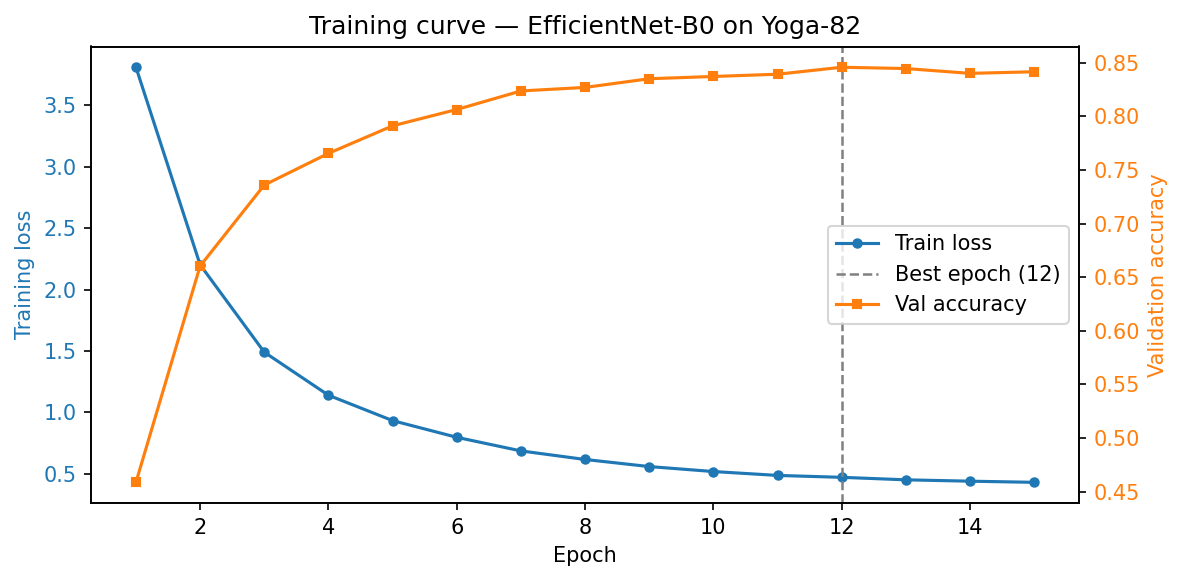
\includegraphics[width=\columnwidth]{fig_training_curve.png}}
\caption{Training loss (left axis) and validation accuracy (right axis) per epoch. The vertical dashed line marks the best checkpoint at epoch~12 (val\_acc $= 0.8457$).}
\label{fig:training}
\end{figure}

\subsection{Test Set Performance}

Table~\ref{tab:results} reports overall metrics on the held-out test set. The model achieves \textbf{85.09\%} top-1 accuracy and a macro-averaged F1 score of \textbf{0.84}, indicating strong per-class performance even across the long tail of rare poses.

\begin{table}[htbp]
\caption{Test set classification metrics}
\begin{center}
\begin{tabular}{|l|c|c|c|c|}
\hline
\textbf{} & \textbf{Precision} & \textbf{Recall} & \textbf{F1} & \textbf{Accuracy} \\
\hline
Macro avg    & 0.85 & 0.84 & 0.84 & -- \\
Weighted avg & 0.86 & 0.85 & 0.85 & -- \\
Overall      &  --  &  --  &  --  & 0.8509 \\
\hline
\end{tabular}
\label{tab:results}
\end{center}
\end{table}

\subsection{Per-Class Analysis}

\begin{figure*}[p]
\centerline{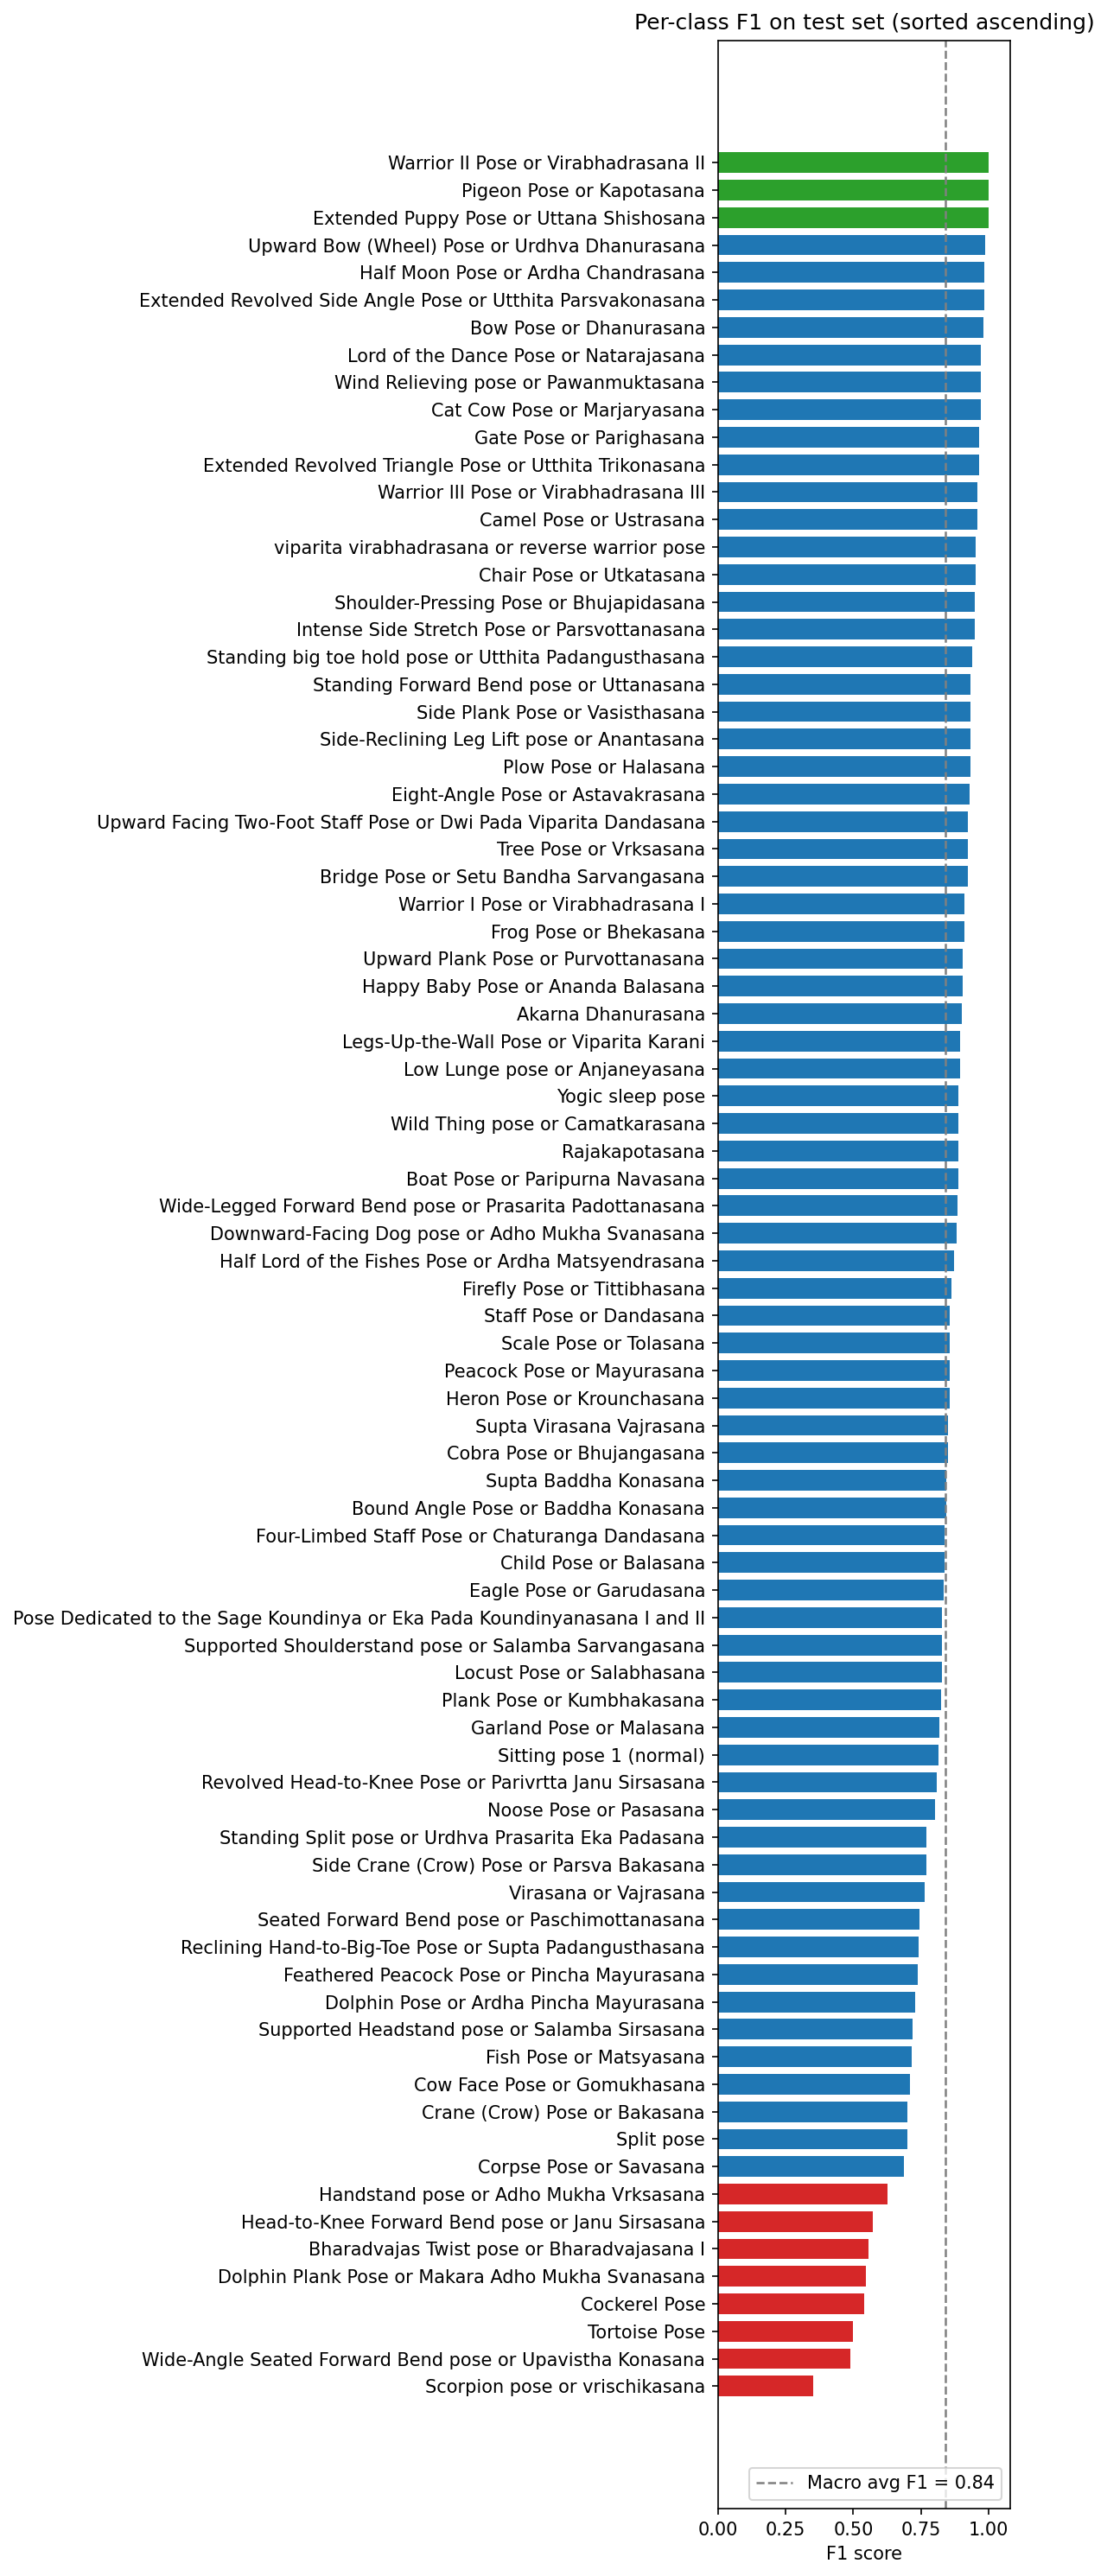
\includegraphics[height=0.92\textheight,keepaspectratio]{fig_f1_per_class.png}}
\caption{Per-class F1 scores on the test set, sorted in ascending order. Red bars highlight the 10 weakest classes; green bars highlight perfect-F1 classes.}
\label{fig:f1_per_class}
\end{figure*}

% FIGURE NEEDED: fig_f1_per_class.png
% Plot: horizontal bar chart — one bar per class (82 bars), sorted ascending by F1.
%        Color the lowest 10 bars red and any bar at F1=1.0 green.
%        Use abbreviated class names on the y-axis.
% All F1 values available from classification_report output in notebook cell ea3351cd.

Fig.~\ref{fig:f1_per_class} shows the full per-class F1 distribution. Several classes achieve perfect F1 scores, including \textit{Extended Puppy Pose}, \textit{Warrior II}, and \textit{Pigeon Pose}. Table~\ref{tab:weak} lists the 10 lowest-F1 classes.

\begin{table}[htbp]
\caption{Ten weakest classes by F1 score on the test set}
\begin{center}
\begin{tabular}{|l|c|c|c|c|}
\hline
\textbf{Class} & \textbf{Prec.} & \textbf{Rec.} & \textbf{F1} & \textbf{N} \\
\hline
Scorpion pose              & 0.60 & 0.25 & 0.35 & 12 \\
Wide-Angle Seated Fwd Bend & 0.50 & 0.48 & 0.49 & 23 \\
Tortoise Pose              & 0.50 & 0.50 & 0.50 & 18 \\
Cockerel Pose              & 0.58 & 0.50 & 0.54 & 14 \\
Dolphin Plank Pose         & 0.50 & 0.60 & 0.55 &  5 \\
Bharadvaja's Twist         & 0.56 & 0.56 & 0.56 &  9 \\
Head-to-Knee Forward Bend  & 0.56 & 0.59 & 0.57 & 17 \\
Handstand                  & 0.52 & 0.80 & 0.63 & 20 \\
Corpse Pose (Savasana)     & 0.57 & 0.85 & 0.69 & 27 \\
Split Pose                 & 0.88 & 0.58 & 0.70 & 38 \\
\hline
\end{tabular}
\label{tab:weak}
\end{center}
\end{table}

Several patterns emerge. Classes with very few test samples (\textit{Dolphin Plank Pose}, $N=5$; \textit{Bharadvaja's Twist}, $N=9$) are sensitive to individual misclassifications. Poses that share body configurations with other classes are also challenging: \textit{Scorpion Pose} and \textit{Handstand} both involve inverted body orientation; \textit{Corpse Pose} (lying flat) overlaps visually with other supine poses; \textit{Head-to-Knee Forward Bend} resembles \textit{Seated Forward Bend}.

\subsection{Confusion Matrix}

% FIGURE NEEDED: fig_confusion_matrix.png
% Plot: 82x82 heatmap using seaborn/matplotlib. Use a log-normalized color scale
%        to make off-diagonal errors visible despite large diagonal dominance.
%        Optionally, instead of (or in addition to) the full matrix, show a
%        "top confused pairs" bar chart listing the 20 most common misclassification
%        pairs by raw count — this is more readable in a two-column paper format.
% The confusion matrix object `cm` is already computed in notebook cell ea3351cd.

\begin{figure}[htbp]
\centerline{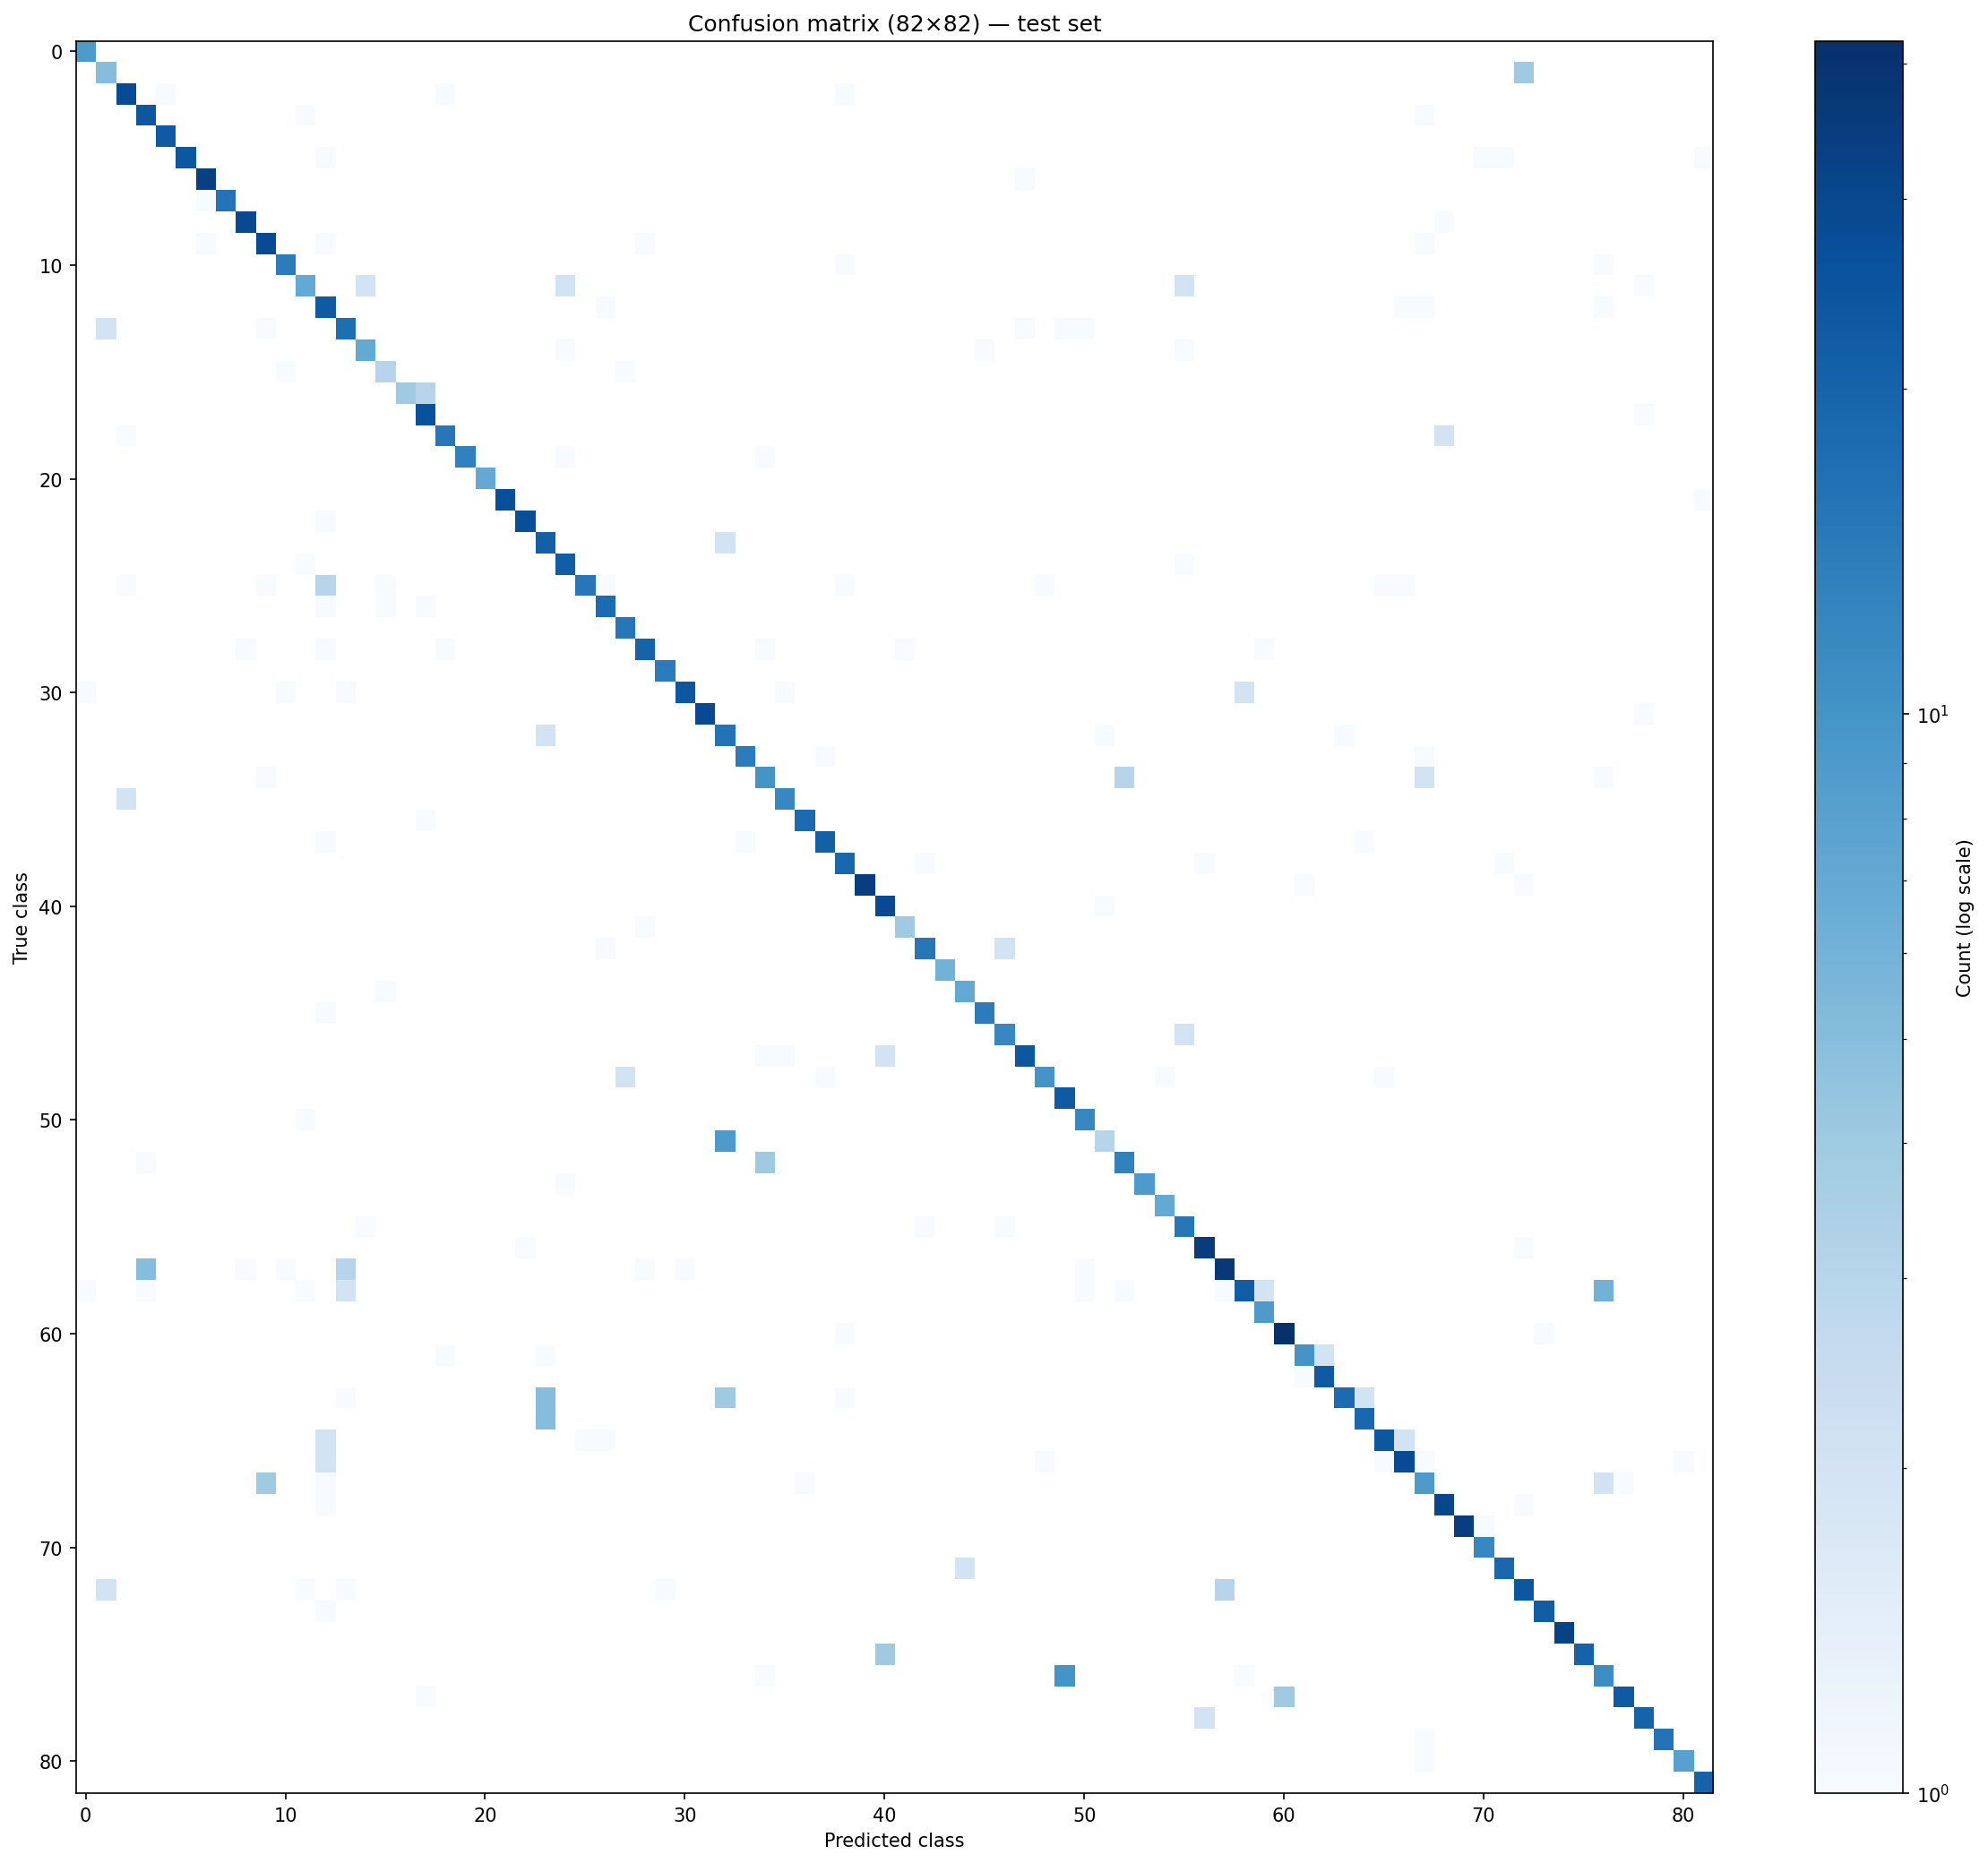
\includegraphics[width=\columnwidth]{fig_confusion_matrix.png}}
\caption{Confusion matrix on the 1{,}764 test images (82$\times$82). Log-normalized color scale; diagonal entries correspond to correct predictions.}
\label{fig:confusion}
\end{figure}

Fig.~\ref{fig:confusion} shows the full confusion matrix. The dominant diagonal confirms strong per-class accuracy. Off-diagonal concentrations reveal the most common error patterns, particularly among structurally similar poses.

\subsection{Image Retrieval}

% FIGURE NEEDED: fig_retrieval.png
% Plot: export the 1x6 figure already generated in notebook cell 8eafe3de
%        (query image + top-5 nearest neighbors with cosine similarity scores).
%        Save as fig_retrieval.png using plt.savefig('fig_retrieval.png', dpi=150, bbox_inches='tight')
%        before plt.show().

\begin{figure}[htbp]
\centerline{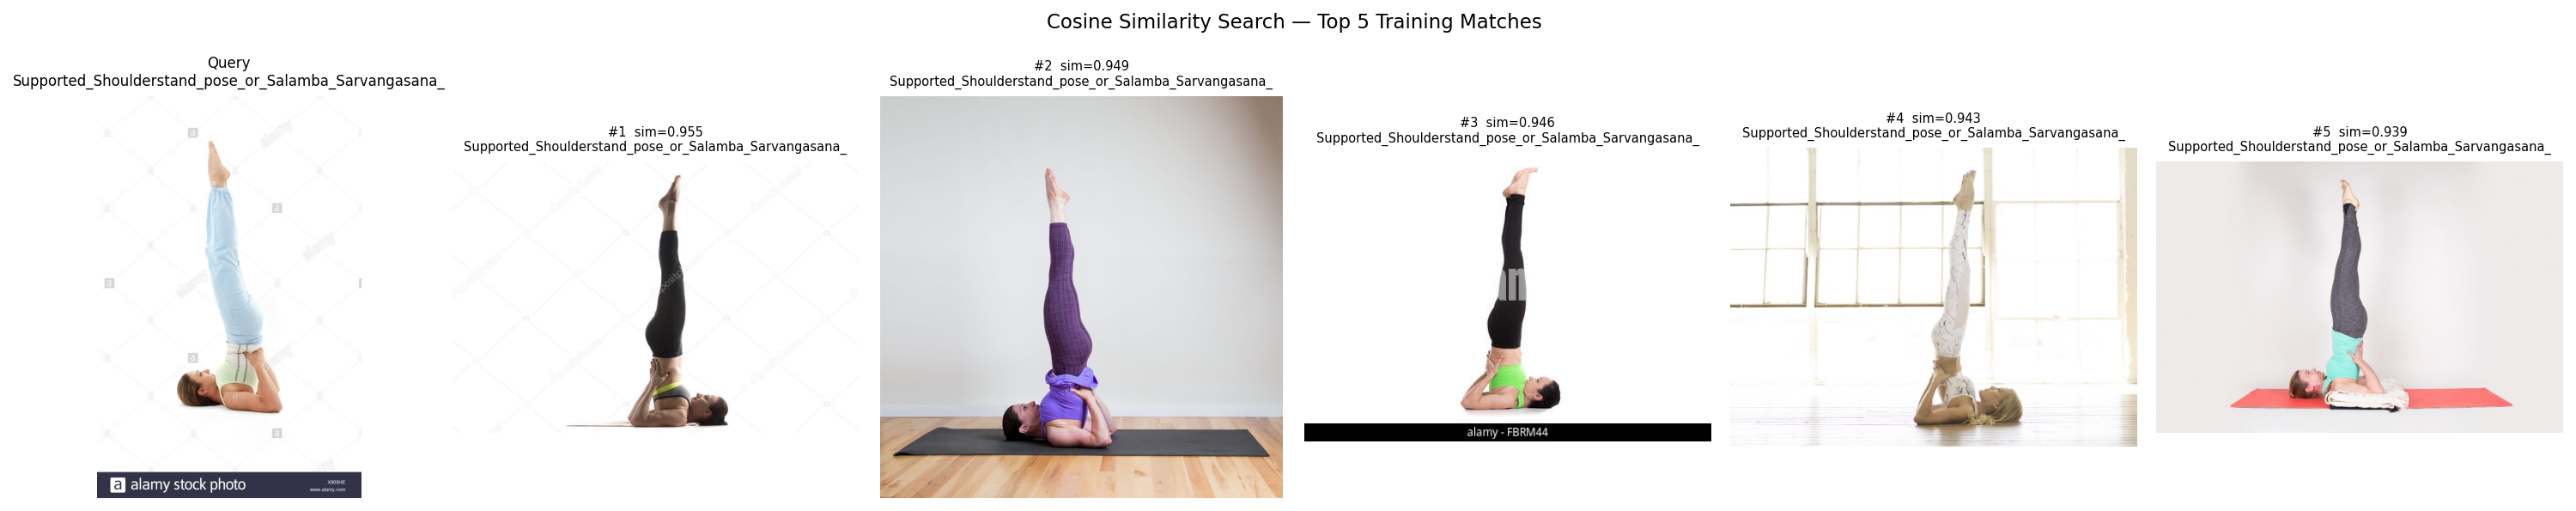
\includegraphics[width=\columnwidth]{fig_retrieval.png}}
\caption{Cosine similarity retrieval. Leftmost image is the query; the five remaining images are the top-5 nearest training neighbors with their cosine similarity scores and class labels.}
\label{fig:retrieval}
\end{figure}

Fig.~\ref{fig:retrieval} shows an example retrieval result. The top-5 nearest training images retrieved by cosine similarity of the 1280-d EfficientNet-B0 embeddings consistently depict the same or closely related pose, confirming that the learned feature space captures semantically meaningful structure.


\section{Conclusions}

We presented an EfficientNet-B0 transfer learning approach to yoga pose classification on Yoga-82, achieving 85.09\% test accuracy and macro F1 of 0.84 across 82 classes without architectural modifications beyond head replacement. Class-weighted loss, cosine annealing scheduling, and data augmentation were key contributors to this result. Analysis of per-class performance shows that visually ambiguous poses and classes with limited test support remain the primary failure modes. The embedding-based retrieval system demonstrates that the model learns semantically coherent representations of pose space. Future work could explore contrastive or metric learning objectives, pose-aware augmentation (skeletal-structure-consistent flips), or hierarchical classification exploiting the semantic hierarchy of Yoga-82 to improve performance on the long tail of difficult poses.

\FloatBarrier
\bibliographystyle{IEEEtran}
\bibliography{saltiniai}

\end{document}
